\begin{frame}[plain]
  {Outline}

  \begin{itemize}
    \item The Keras
    \item Neural network flow with Keras
    \item Deep neural network
    \item Flexible interface
  \end{itemize}
\end{frame}

\begin{frame}[plain]
  {Keras}

  %%%Text area
  Keras is a high-level neural networks API, written in Python and capable of running on top of TensorFlow, CNTK, or Theano.
  
  It was developed with a focus on enabling fast experimentation.
  
  Being able to go from idea to result with the least possible delay is key to doing good research.

  Their features:
  \begin{itemize}
    \item Allows for easy and fast prototyping (through user friendliness, modularity, and extensibility).
    \item Supports both convolutional networks and recurrent networks, as well as combinations of the two.
    \item Runs seamlessly on CPU and GPU.
  \end{itemize}
\end{frame}

\begin{frame}[plain]
  {Neural network model constraction}

  \begin{figure}
    \centering
    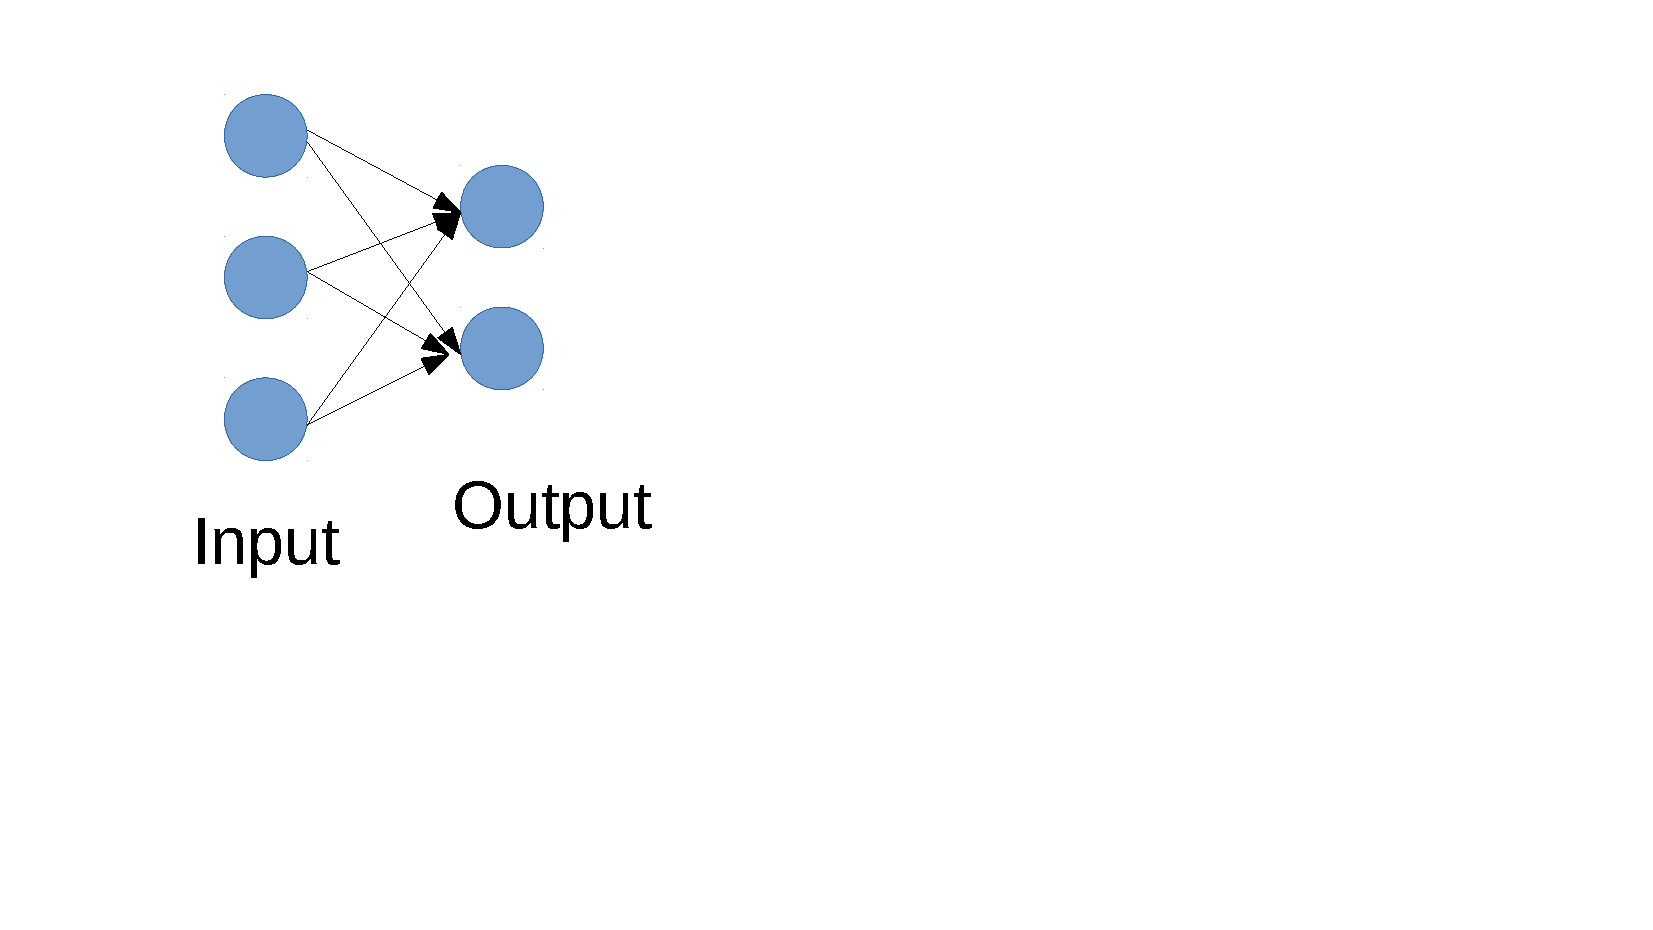
\includegraphics[height=2.5cm]{keras.pdf}
    \caption{Full connected (Dense) single-layer neural net}
  \end{figure}
  \lstinputlisting[caption=model definition]{keras_sample.py}
\end{frame}

\begin{frame}[plain]
  {Train the model}

  \lstinputlisting[caption=model compile and fit]{train.py}
\end{frame}

\begin{frame}[plain]
  {Deep neural network}

  \begin{figure}
    \centering
    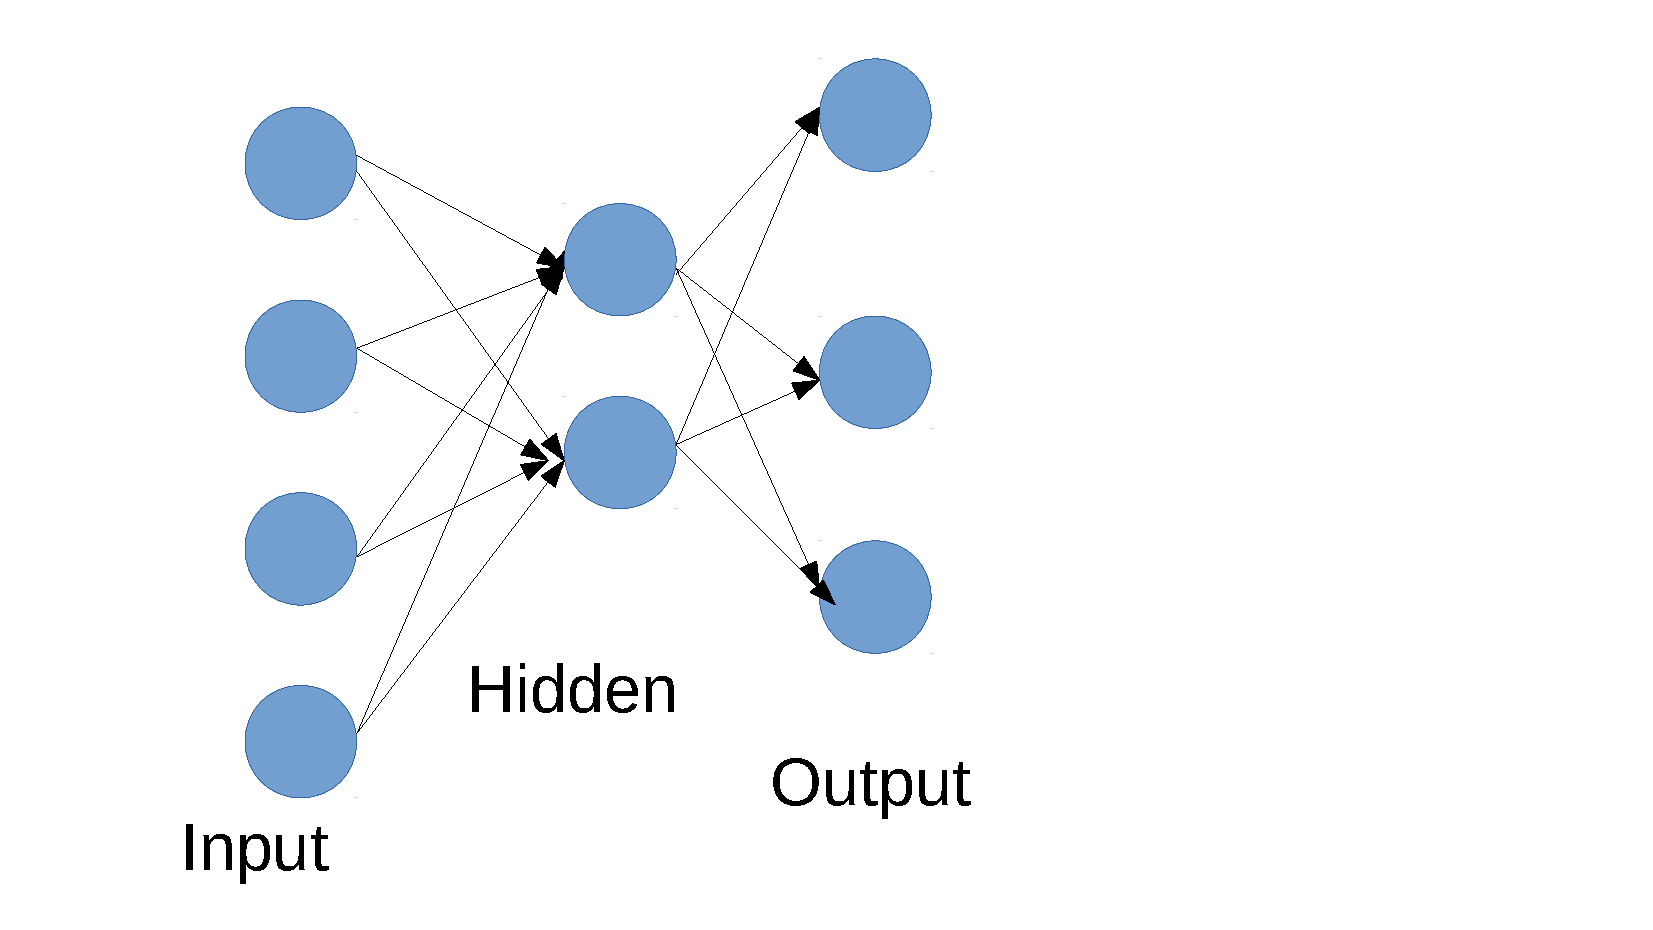
\includegraphics[width=5cm]{multi.pdf}
    \caption{Full connected (Dense) hidden-layer neural network}
  \end{figure}
  \lstinputlisting[caption=Deep neural net definition]{multi.py}
\end{frame}

\begin{frame}[plain]
  {Second interface}

  \lstinputlisting[caption=Deep neural net definition]{multi.py}
  Oneline

  \lstinputlisting[caption=Deep neural net definition]{multi2.py}
  Multi line
\end{frame}

\begin{frame}[plain]
  {Practical multiline interface}

  \begin{figure}
    \centering
    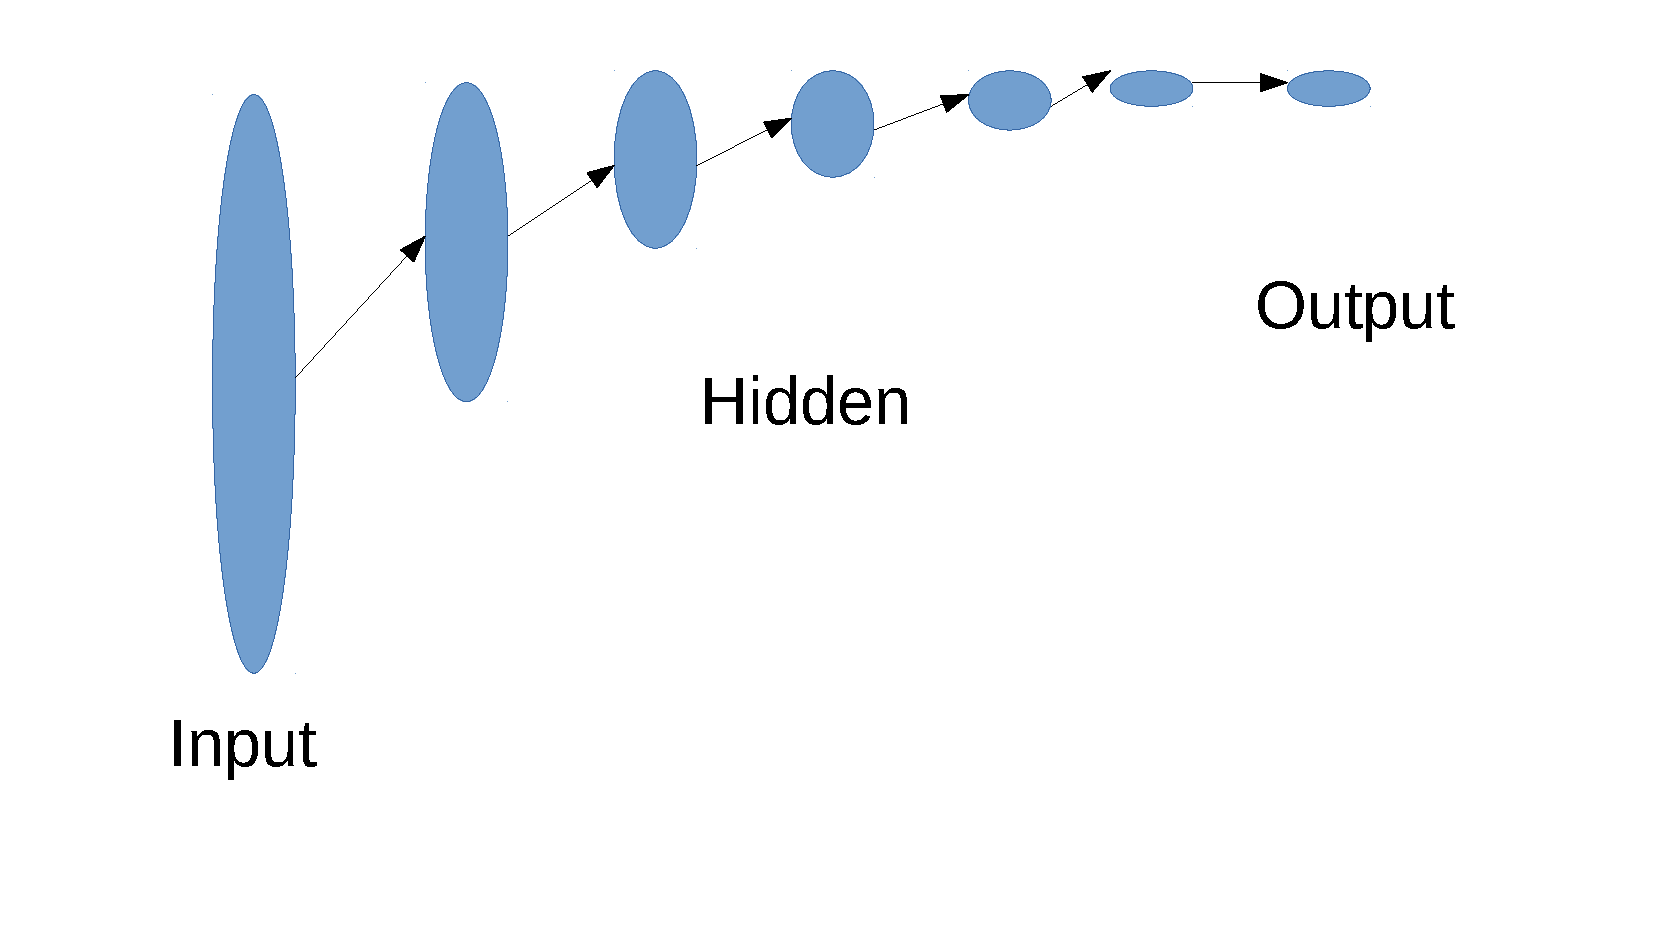
\includegraphics[height=2.3cm]{practical.pdf}
    \caption{Practical network}
  \end{figure}
  \lstinputlisting[caption=Deep neural net definition]{practical_multi_line.py}
\end{frame}
